\documentclass[12pt, twoside]{article}
\usepackage[letterpaper, margin=1in, head=30pt, headsep=0.1in]{geometry}
\usepackage[english]{babel}
\usepackage[utf8]{inputenc}
\usepackage{amsmath}
\usepackage{amsfonts}
\usepackage{amssymb}
\usepackage{tikz}
\usepackage{yhmath} %arcs using \wideparen{}
\usetikzlibrary{quotes, angles}

\usepackage{graphicx}
\usepackage{enumitem}
\usepackage{multicol}

%\usepackage{pgfplots}
%\pgfplotsset{width=10cm,compat=1.9}
%\usepgfplotslibrary{statistics}
%\usepackage{pgfplotstable}
%\usepackage{tkz-fct}
%\usepackage{venndiagram}

\usepackage{fancyhdr}
\pagestyle{fancy}
\fancyhf{}
\renewcommand{\headrulewidth}{0pt} % disable the underline of the header
\raggedbottom
\newif\ifmeta
\metatrue %print standards and topics tags

\title{High School Geometry problem sets}
\author{Chris Huson}
\date{April 2021}

%\fancyhead[RE]{\thepage}
%\fancyhead[RO]{\thepage \\ Name: \hspace{3cm}}
%\fancyhead[L]{BECA / Dr. Huson / 10th Grade Geometry\\* 7 June 2019}
%
%\begin{document}
%\subsubsection*{13.7 Homework: Cross sections, distance applications}
%\fancyhead[L]{BECA / Dr. Huson / Geometry 03-Volume+angle-bisectors\\* pset ID: 34}

\begin{document}

\subsubsection*{8.1 Radians}
\begin{enumerate}
\item Do Now: Given circle $O$ with $m\angle ACB=40^\circ$.
  \begin{multicols}{2}
    \raggedcolumns
    \begin{enumerate}
      \item Find the $m \wideparen{AB}$. \vspace{2cm}
      \item Write down the $m\angle AOB$. \vspace{1.7cm}
    \end{enumerate}
      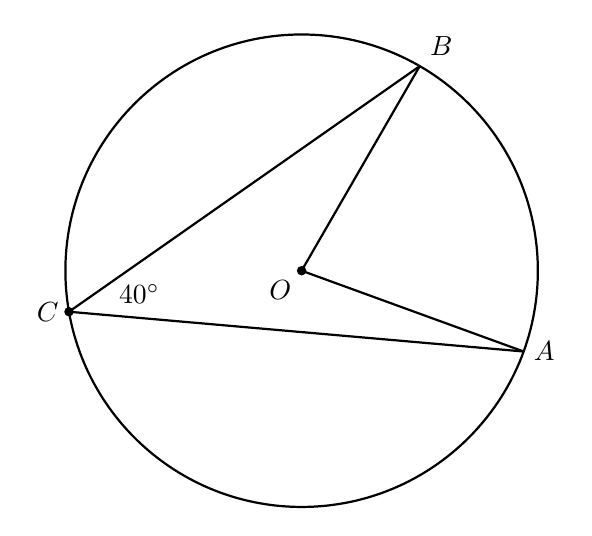
\begin{tikzpicture}[scale=.6, rotate=0]
        \draw [thick] (0,0) circle[radius=5];
        \fill (0,0) circle[radius=.1];
        \draw [thick]
        (-20:5) node[right] {$A$}--
        (0,0) node[below left] {$O$}--
        (60:5) node[above right] {$B$};
        \draw [thick] (-20:5)--(190:5) node[left] {$C$}--(60:5);
        \fill (190:5) circle[radius=.1];
        \draw (187:4.1) node[right]{$40^\circ$};
      \end{tikzpicture}
  \end{multicols}

\newpage
\item Do Now: A \emph{unit} circle with a radius $r=1$ is divided in quarters. One sector, $AOB$, is shaded as shown.
  \begin{multicols}{2}
  \raggedcolumns
  \begin{enumerate}[itemsep=1.5cm]
    \item Find the circumference in terms of $\pi$. ($C=2\pi r$)
    \item Write down $m \angle AOB$ in \emph{degrees}.
    \item Find the \emph{length} of the arc $\wideparen{AB}$ in terms of $\pi$.
  \end{enumerate}
  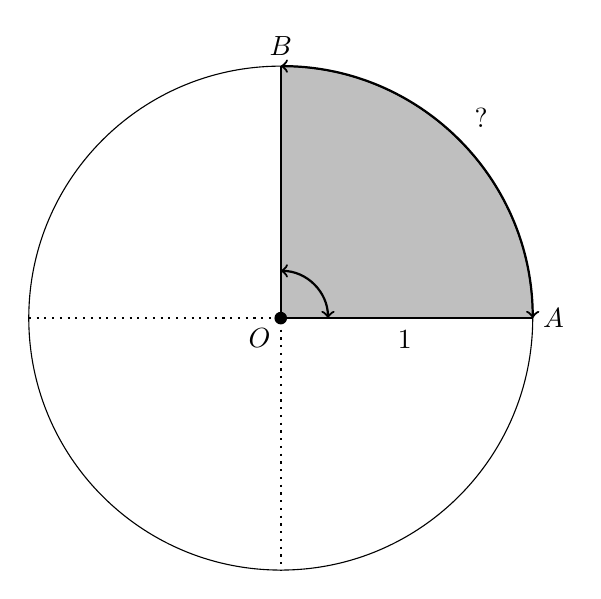
\begin{tikzpicture}[scale=0.8]
    \fill [lightgray]
    (0,0)--(0:4) arc (0:90:4)--(0,0);
    \draw (0,0) circle[radius=4];
    \draw [thick, <->] (0:0.75) arc (0:90:0.75);
    \draw [thick, <->] (0:4) arc (0:90:4);
    \draw [thick]
    (0:4) node[right] {$A$}--
    (0,0) node[below left] {$O$}--
    (90:4) node[above] {$B$};
    \draw [thick, dotted](0:-4)--(0,0)--(-90:4);
    \fill (0,0) circle[radius=.1];
    \node at (45:4.5) {$?$};
    \node at (-10:2) {$1$};
  \end{tikzpicture}
  \end{multicols}

\newpage
\item Groupwork warmup: Write the names of the people in your group and fill in the table\\[0.25cm]
Group order: shortest first name to longest
\begin{multicols}{2}  
  \begin{enumerate}
    \item Group members:
    \item On the left write down your favorite fruit and condiment.
    \item Write the group consensus favorite fruit and condiment.
    \end{enumerate}
  \begin{tikzpicture}[scale=0.7, rotate=0]
  \draw [thick] (-5,0)--(5,0);
  \draw [thick] (0,-4)--(0,4);
  \node at (-4,4){Fruit};
  \node at (-3.5,-0.5){Condiment};
\end{tikzpicture}
\end{multicols}
(condiments are ketchup, mustard, salt, sugar, honey, whipped cream, etc.)

\newpage
\item Groupwork challenge: Each member picks a different color and Greek letter, writing it in the upper left quadrant.\\[0.25cm]
Display screen and copy/paste each team member's letter into a different quadrant.
\begin{center}
  \begin{tikzpicture}[scale=1, rotate=0]
  \draw [thick] (-5,0)--(5,0);
  \draw [thick] (0,-4)--(0,4);
  \node at (-4,4){Your letter:};
\end{tikzpicture}
\end{center}
Example Greek letters are 
{\Large$\pi$, $\theta$, $\alpha$, $\Delta$, $\beta$ \par}
Group order: longest last name to shortest

\newpage
\item Lesson: The length of the arc of a unit circle is a measure of the central angle called \emph{radians}. The circumference of the full circle is $2 \pi = 360^\circ$.\\[0.25cm]
Mark each angle with its radian measure.
  \begin{multicols}{2}
  \raggedcolumns
  \begin{enumerate}
    \item One half of a circle $180^\circ$\\
    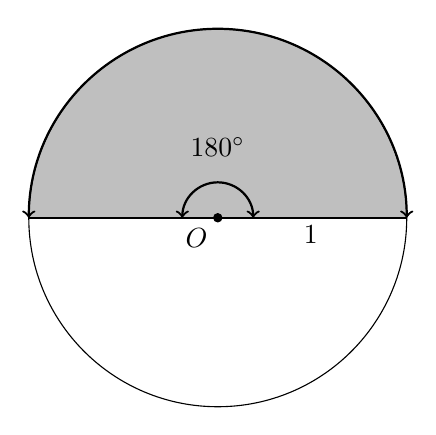
\begin{tikzpicture}[scale=0.6]
      \fill [lightgray]
      (0,0)--(0:4) arc (0:180:4)--(0,0);
      \draw (0,0) circle[radius=4];
      \draw [thick, <->] (0:0.75) arc (0:180:0.75);
      \draw [thick, <->] (0:4) arc (0:180:4);
      \draw [thick]
      (0:4)--(0,0) node[below left] {$O$}--(180:4);
      %\draw [thick, dotted](0:-4)--(0,0)--(120:4);
      \fill (0,0) circle[radius=.1];
      \node at (90:1.5) {$180^\circ$};
      \node at (-10:2) {$1$};
    \end{tikzpicture}
    \item One sixth of the circle $60^\circ$\\
    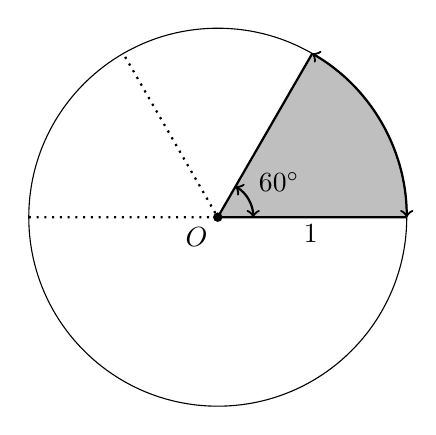
\begin{tikzpicture}[scale=0.6]
      \fill [lightgray]
      (0,0)--(0:4) arc (0:60:4)--(0,0);
      \draw (0,0) circle[radius=4];
      \draw [thick, <->] (0:0.75) arc (0:60:0.75);
      \draw [thick, <->] (0:4) arc (0:60:4);
      \draw [thick]
      (0:4)--(0,0) node[below left] {$O$}--(60:4);
      \draw [thick, dotted](0:-4)--(0,0)--(120:4);
      \fill (0,0) circle[radius=.1];
      \node at (30:1.5) {$60^\circ$};
      \node at (-10:2) {$1$};
    \end{tikzpicture}
    \item One eighth of the circle $45^\circ$\\
    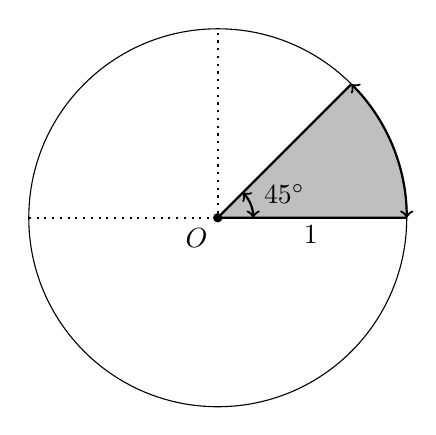
\begin{tikzpicture}[scale=0.6]
      \fill [lightgray]
      (0,0)--(0:4) arc (0:45:4)--(0,0);
      \draw (0,0) circle[radius=4];
      \draw [thick, <->] (0:0.75) arc (0:45:0.75);
      \draw [thick, <->] (0:4) arc (0:45:4);
      \draw [thick]
      (0:4)--(0,0) node[below left] {$O$}--(45:4);
      \draw [thick, dotted](0:-4)--(0,0)--(90:4);
      \fill (0,0) circle[radius=.1];
      \node at (20:1.5) {$45^\circ$};
      \node at (-10:2) {$1$};
    \end{tikzpicture}
    \item One third of a circle $120^\circ$\\
    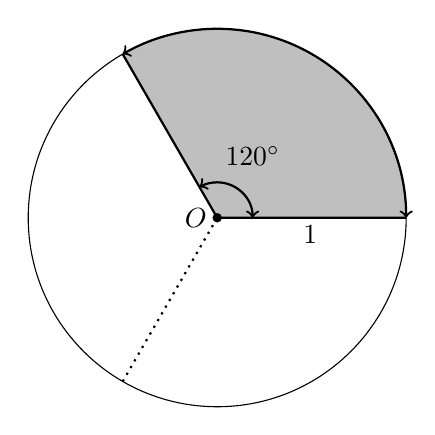
\begin{tikzpicture}[scale=0.6]
      \fill [lightgray]
      (0,0)--(0:4) arc (0:120:4)--(0,0);
      \draw (0,0) circle[radius=4];
      \draw [thick, <->] (0:0.75) arc (0:120:0.75);
      \draw [thick, <->] (0:4) arc (0:120:4);
      \draw [thick]
      (0:4)--(0,0) node[left] {$O$}--(120:4);
      \draw [thick, dotted](240:4)--(0,0);
      \fill (0,0) circle[radius=.1];
      \node at (60:1.5) {$120^\circ$};
      \node at (-10:2) {$1$};
    \end{tikzpicture}
  \end{enumerate}
  \end{multicols}

\newpage
\item Lesson: Algebra view of \emph{radians} to \emph{degrees} using the formula $2 \pi = 360^\circ$ or $\pi = 180^\circ$.\\[0.25cm]
Apply the appropriate formula.
\begin{multicols}{2}
$\displaystyle r = d \times \frac{\pi}{180}$\\
$\displaystyle d = r \times \frac{180}{\pi}$
\end{multicols}
  \begin{multicols}{2}
  \raggedcolumns
  \begin{enumerate}
    \item $60^\circ = \hspace{0.15cm} ?$ radians\\[0.5cm]
    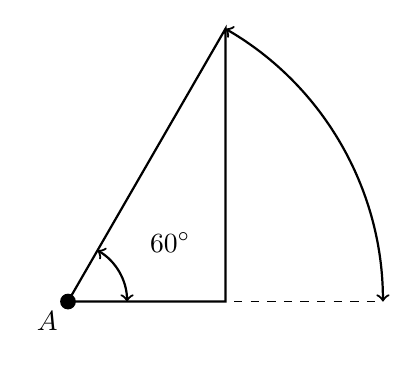
\begin{tikzpicture}[scale=1]
      \draw [thick, <->] (0:0.75) arc (0:60:0.75);
      \draw [thick, <->] (0:4) arc (0:60:4);
      \draw [dashed](0,0)--(4,0);
      \draw [thick]
      (0,0) node[below left] {$A$}--(60:4)--(2,0)--cycle;
      \fill (0,0) circle[radius=.1];
      \node at (30:1.5) {$60^\circ$};
    \end{tikzpicture}
    \item $30^\circ = \hspace{0.15cm} ?$ radians\\[0.5cm]
    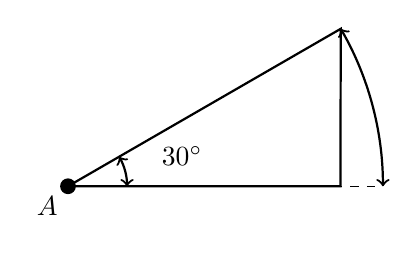
\begin{tikzpicture}[scale=1]
      \draw [thick, <->] (0:0.75) arc (0:30:0.75);
      \draw [thick, <->] (0:4) arc (0:30:4);
      \draw [dashed](0,0)--(4,0);
      \draw [thick]
      (0,0) node[below left] {$A$}--(30:4)--(3.46,0)--cycle;
      \fill (0,0) circle[radius=.1];
      \node at (15:1.5) {$30^\circ$};
    \end{tikzpicture}
    \item $\displaystyle \frac{\pi}{4}  = \hspace{0.15cm} ?$ degrees\\[0.5cm]
    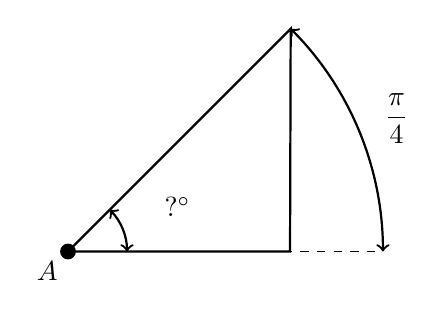
\begin{tikzpicture}[scale=1]
      \draw [thick, <->] (0:0.75) arc (0:45:0.75);
      \draw [thick, <->] (0:4) arc (0:45:4);
      \draw [dashed](0,0)--(4,0);
      \draw [thick]
      (0,0) node[below left] {$A$}--(45:4)--(2.82,0)--cycle;
      \fill (0,0) circle[radius=.1];
      \node at (22:1.5) {$?^\circ$};
      \node at (22:4.5) {$\displaystyle \frac{\pi}{4}$};
    \end{tikzpicture}
    \item $\displaystyle \frac{\pi}{8}  = \hspace{0.15cm} ?$ degrees\\[0.75cm]
    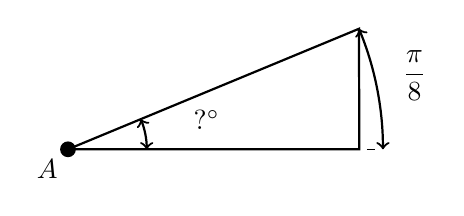
\begin{tikzpicture}[scale=1]
      \draw [thick, <->] (0:1) arc (0:22.5:1);
      \draw [thick, <->] (0:4) arc (0:22.5:4);
      \draw [dashed](0,0)--(4,0);
      \draw [thick]
      (0,0) node[below left] {$A$}--(22.5:4)--(3.7,0)--cycle;
      \fill (0,0) circle[radius=.1];
      \node at (12:1.8) {$?^\circ$};
      \node at (12:4.5) {$\displaystyle \frac{\pi}{8}$};
    \end{tikzpicture}
  \end{enumerate}
  \end{multicols}

\newpage
\item Right $\triangle ABC$ is drawn in \emph{standard position} with vertex $A$ on the origin and right $\angle C$ on the $x$-axis, as shown.
\begin{multicols}{2}
  \raggedcolumns
\begin{enumerate}
  \item Find the length of the hypotenuse $AB$ using the Pythagorean Theorem $a^2 + b^2 = c^2$. (leave as a radical)
  \vspace{3cm}
  \item Find the slope of the line segment $\overline{AB}$ as a decimal.
\end{enumerate}
  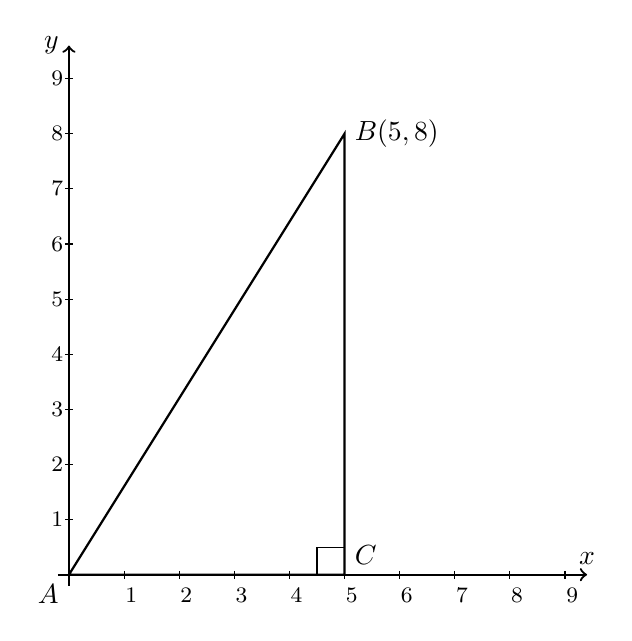
\begin{tikzpicture}[scale=0.7]
    %\draw [help lines] (-1.15,-1.2) grid (11,10);
    \draw [thick, ->] (-0.2,0) -- (9.4,0) node [above] {$x$};
    \foreach \x in {1,2,...,9}
      \draw[shift={(\x,0)},color=black] (0pt,2pt) -- (0pt,-2pt) node[below] {\footnotesize \; $\x$};
    \draw [thick, ->] (0,-0.2)--(0,9.6) node [left] {$y$};
    \foreach \y in {1,2,...,9}
      \draw[shift={(0,\y)},color=black] (-2pt,0pt) -- (2pt,0pt) node[left] {\footnotesize \; $\y$};
    \draw [-, thick] (0,0) node[below left] {$A$}
    --(5,0) node[above right] {$C$}
    --(5,8)node[right] {$B (5,8)$}--cycle;
    \draw (5,0)++ (-0.5,0)-- +(0,0.5)-- +(0.5,0.5);
    %\draw [<->, thick] (-0.6,4.3)--(5,8.5);
  \end{tikzpicture}
\end{multicols}


\end{enumerate}
\end{document}